%%%%%%%%%%%%%%%%%%%%%%% file template.tex %%%%%%%%%%%%%%%%%%%%%%%%%
%
% This is a general template file for the LaTeX package SVJour3
% for Springer journals.          Springer Heidelberg 2010/09/16
%
% Copy it to a new file with a new name and use it as the basis
% for your article. Delete % signs as needed.
%
% This template includes a few options for different layouts and
% content for various journals. Please consult a previous issue of
% your journal as needed.
%
%%%%%%%%%%%%%%%%%%%%%%%%%%%%%%%%%%%%%%%%%%%%%%%%%%%%%%%%%%%%%%%%%%%
%
% First comes an example EPS file -- just ignore it and
% proceed on the \documentclass line
% your LaTeX will extract the file if required
\begin{filecontents*}{example.eps}
%!PS-Adobe-3.0 EPSF-3.0
%%BoundingBox: 19 19 221 221
%%CreationDate: Mon Sep 29 1997
%%Creator: programmed by hand (JK)
%%EndComments
gsave
newpath
  20 20 moveto
  20 220 lineto
  220 220 lineto
  220 20 lineto
closepath
2 setlinewidth
gsave
  .4 setgray fill
grestore
stroke
grestore
\end{filecontents*}
%
\RequirePackage{fix-cm}
%
%\documentclass{svjour3}                     % onecolumn (standard format)
%\documentclass[smallcondensed]{svjour3}     % onecolumn (ditto)
\documentclass[smallextended,natbib]{svjour3}       % onecolumn (second format)
%\documentclass[twocolumn]{svjour3}          % twocolumn
%
\smartqed  % flush right qed marks, e.g. at end of proof
%
\usepackage{graphicx}
%
% \usepackage{mathptmx}      % use Times fonts if available on your TeX system
%
% insert here the call for the packages your document requires
%\usepackage{latexsym}
% etc.
%
% please place your own definitions here and don't use \def but
% \newcommand{}{}
%
% Insert the name of "your journal" with
% \journalname{myjournal}
%
\begin{document}

\title{A Fast Algorithm for Node-Centric Betweenness Centrality%\thanks{Grants or other notes
%about the article that should go on the front page should be
%placed here. General acknowledgments should be placed at the end of the article.}
}
%\subtitle{Do you have a subtitle?\\ If so, write it here}

%\titlerunning{Short form of title}        % if too long for running head

\author{First Author         \and
        Second Author %etc.
}

%\authorrunning{Short form of author list} % if too long for running head

\institute{F. Author \at
              first address \\
              Tel.: +123-45-678910\\
              Fax: +123-45-678910\\
              \email{fauthor@example.com}           %  \\
%             \emph{Present address:} of F. Author  %  if needed
           \and
           S. Author \at
              second address
}

\date{Received: date / Accepted: date}
% The correct dates will be entered by the editor


\maketitle

\begin{abstract}
Insert your abstract here. Include keywords, PACS and mathematical
subject classification numbers as needed.
\keywords{First keyword \and Second keyword \and More}
% \PACS{PACS code1 \and PACS code2 \and more}
% \subclass{MSC code1 \and MSC code2 \and more}
\end{abstract}

\section{Introduction}
\label{intro}
A social network consists of a set of actors, like persons or organizations, and one or more types of relations between them. 
Betweenness is a popular measure of centrality investigated in the context of social network analysis. 
Betweenness of an actor indicates the extent to which the actor is between all other actors within a given social network, and it expresses the importance and influence of the actor in the social network \citep{centrality}.

Calculating the betweenness of each node, however, requires finding all of the shortest paths between every pair of nodes in the given network.
Since carrying out this task in a large network will incur prohibitively expensive computational costs, a large amount of research for estimating betweenness have been carried out. Although the estimating techniques efficiently estimate the betweenness measure with a low error margin, the exact betweenness calculation of only one node is still    
In these techniques  \citep{SIMBET,egocentric,everett,ICCN:lbcdna,Pant13:Local}, each node identifies its \emph{ego network}, a logical network consisting of that node, its 1-hop neighbors, and all links between these nodes.
Then, each node calculates, as an estimate of its betweenness in the entire network, its betweenness only in its ego network, thereby saving both network and computational resources.


\section{Problem Definition and Related Work}
In this paper, we consider a graph $G(V, E)$ where $V$ is a set of vertices and $E$ is a set of undirected and unweighted edges representing social links between vertices\footnote{We use the term {\em actors} and {\em social links} to refer to individuals, groups or organizations and their relationships in a social network. On the other hand, the graph representing a social network consists of {\em vertices} and {\em edges} representing actors and social links, respectively.}. Given a graph $G(V, E)$, the betweenness $B(v)$ of a vertex $v$ is defined as:
\begin{equation}\label{bet}
B(v) = \frac{\sum_{s \neq v \neq t \in V}\frac{\sigma_{st}(v)}{\sigma_{st}}}{(|V|-1)(|V|-2)}
\end{equation} where $\sigma_{st}$ is the number of shortest paths from vertex $s$ to vertex $t$ and $\sigma_{st}(v)$ is the number of those shortest paths that pass through vertex $v$. 
In the above definition, the denominator represents the total number of pairs of all vertices except $v$, and normalizes $B(v)$ to a value between 0 and 1. Given an undirected graph, $\sigma_{st}=\sigma_{ts}$ and $\sigma_{st}(v)=\sigma_{ts}(v)$ for all vertices $s$, $t$, and $v$, so that it is sufficient to find either $\sigma_{st}$ or $\sigma_{ts}$ and either $\sigma_{st}(v)$ or $\sigma_{ts}(v)$.

The fastest algorithm for exactly computing the betweenness of every vertex in a given graph is developed by \citet{Brandes01afaster}. Given an unweighted graph, the Brandes algorithm performs a breadth first search to compute the number of shortest paths from any pair of two vertices. It then derives the betweenness of each vertex by aggregating the previously computed count values backwards along the edges. Given an unweighted graph $G(V,E)$, this Brandes algorithm takes $O(|V||E|)$ time.

Since the exact calculation of the betweenness even for a single vertex involves the computation of the shortest path between any pair of vertexes, a feasible solution is to estimate the betweenness values. Vertex sampling consists in selecting a set of nodes in
a graph \citep{Eppstein:2001:FAC:365411.365449,10.1093/comjnl/bxu003,10.1007/978-3-319-16112-9_11}. The selected nodes are called pivot nodes. The process of sampling the nodes can be fully random or based on a heuristic. Usually, for the purpose of betweenness estimation, the computation of the shortest paths is only executed over the sampled nodes, and the betweenness values are estimated for every vertex in a graph or just for a set of top-class vertexes.

\label{sec:1}
Text with citations \cite{RefB} and \cite{RefJ}.
\subsection{Subsection title}
\label{sec:2}
as required. Don't forget to give each section
and subsection a unique label (see Sect.~\ref{sec:1}).
\paragraph{Paragraph headings} Use paragraph headings as needed.
\begin{equation}
a^2+b^2=c^2
\end{equation}

% For one-column wide figures use
\begin{figure}
% Use the relevant command to insert your figure file.
% For example, with the graphicx package use
  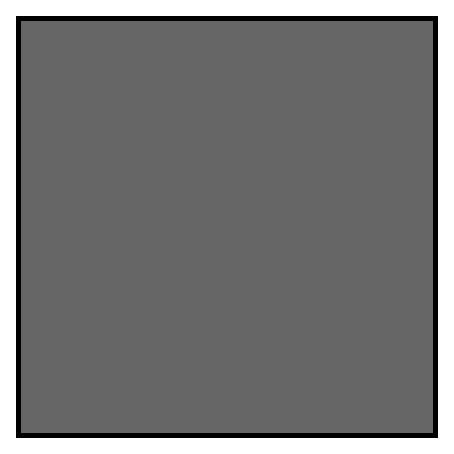
\includegraphics{example.eps}
% figure caption is below the figure
\caption{Please write your figure caption here}
\label{fig:1}       % Give a unique label
\end{figure}
%
% For two-column wide figures use
\begin{figure*}
% Use the relevant command to insert your figure file.
% For example, with the graphicx package use
  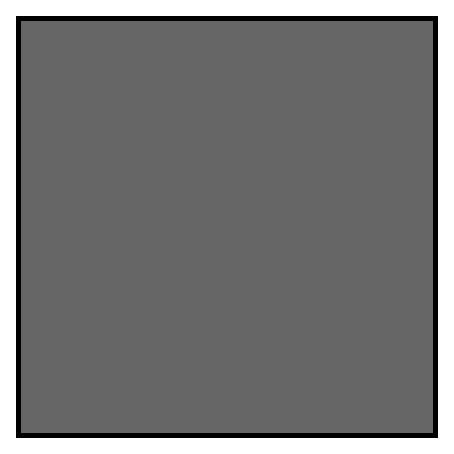
\includegraphics[width=0.75\textwidth]{example.eps}
% figure caption is below the figure
\caption{Please write your figure caption here}
\label{fig:2}       % Give a unique label
\end{figure*}
%
% For tables use
\begin{table}
% table caption is above the table
\caption{Please write your table caption here}
\label{tab:1}       % Give a unique label
% For LaTeX tables use
\begin{tabular}{lll}
\hline\noalign{\smallskip}
first & second & third  \\
\noalign{\smallskip}\hline\noalign{\smallskip}
number & number & number \\
number & number & number \\
\noalign{\smallskip}\hline
\end{tabular}
\end{table}


%\begin{acknowledgements}
%If you'd like to thank anyone, place your comments here
%and remove the percent signs.
%\end{acknowledgements}

% BibTeX users please use one of
%\bibliographystyle{spbasic}      % basic style, author-year citations
%\bibliographystyle{spmpsci}      % mathematics and physical sciences
%\bibliographystyle{spphys}       % APS-like style for physics
%\bibliography{}   % name your BibTeX data base

% Non-BibTeX users please use
\bibliographystyle{spbasic}
\bibliography{../../LinkPaper}
\end{document}
% end of file template.tex

